\newpage
\section{评估NVIDIA新架构GPU的机器学习应用性能}
\setcounter{table}{0}
\setcounter{figure}{0}
\subsection{实验工具与环境}
\subsubsection{实验环境}
\par 表\ref{table-环境}中列出实验环境。\\
\begin{table}
	\centering
	\renewcommand{\thetable}{\arabic{section}-\arabic{table} }
	\renewcommand{\tablename}{表}
	\caption{实验环境}
	\addtocounter{table}{-1}
	\renewcommand{\thetable}{\arabic{section}-\arabic{table} }
	\renewcommand{\tablename}{Table}
	\caption{Environment}
	\begin{tabular}{cc}
		\toprule
		项目	&	内容\\
		\midrule
		CPU		&	AMD Ryzen ThreadRipper 2990WX 32C64T @ 3.0GHz\\
		主板		&	MSI X399\\
		内存		&	CORSAIR DDR4 3200 @ 16-15-15-15-34-1T 128GB\\
		GPU		&	NVIDIA Geforce RTX 2080TI (Turing)\\
		硬盘		&	INTEL750 NVMe PCIe 1.2TB * 2 @ RAID 0\\
		系统		&	Windows 10 64-bit build 17763\\	
		CUDA	&	10.1, 10.0, 9.2, 9.0\\
		其他		&	Jetson TX2 $ * $\\
		\bottomrule
		$ * $该硬件由NVIDIA提供。\\
	\end{tabular} 
	\label{table-环境}
\end{table}

\subsubsection{实验工具}
\par 实验中使用到了若干软件工具,如表\ref{table-实验工具}列出。
\begin{table}
	\centering
	\renewcommand{\thetable}{\arabic{section}-\arabic{table} }
	\renewcommand{\tablename}{表}
	\caption{实验工具}
	\addtocounter{table}{-1}
	\renewcommand{\thetable}{\arabic{section}-\arabic{table} }
	\renewcommand{\tablename}{Table}
	\caption{Tools}
	\begin{tabular}{cc}
		\toprule
		项目	&	内容\\
		\midrule
		Python 3.6		&	用于进行数据统计、编写TensorFlow应用\\
		Conda 4.5.12		&	用于创建、管理、隔离Python环境\\
		TensorFlow		&	1.12.0和1.13.0版本的源码,用于对比、研究、调整\\
		Bazel 0.16.0		&	用于从源码构建TensorFlow\\
		Msys2		&	用于从源码构建TensorFlow\\
		CMake 3.1.0		&	用于构建CUTLASS\\	
		Nsight 6.0	&	用于后台监听CUDA应用,捕捉Trace\\
		nvprof		&	用于分析CUDA程序的API调用、分支效率等\\
		git			&	版本控制\\
		Perforce	&	版本控制\\
		Ubuntu 16.04 Physical & 用于执行GPGPU-SIM 应用\\
		GPGPU-SIM 3.2 & 用于从指令级别模拟CUDA程序\\
		Visual Studio 2017 & 搭配10.0.17763.0版本的SDK\\
		\bottomrule
	\end{tabular} \label{table-实验工具} 
\end{table}
\subsection{实验详细过程}
\subsubsection{基于测试样例的Benchmark}
\par 为了为接下来的实验设定基准,这一步先使用用途单一的测试样例测试绝对性能以及相应的提升,因不同架构的硬件各项参数(包括流处理器数量、显存容量等)不尽相同,所以直接对比不同架构硬件的性能是没有意义的,这里选择对比不同架构硬件在不同SDK下性能提升的比例。此处选用了CUDA 10.0,CUDA 9.2,CUDA 9.0三种SDK,同时选用9.2与9.0的原因是因为9.2版本是为了图灵架构的GPU Tesla V100发布的\parencite{CUDA92},也在本文的研究范围内。
\par 因为本文主要讨论新架构GPU在机器学习应用中带来的性能提升,故选用的评测样例大部分都与机器学习应用相关;主要从以下角度进行评估:通用矩阵乘法(GEMM, General Matrix Multiply)、矩阵乘法运算性能、卷积运算性能、神经网络推理性能以及结合框架的综合性能。在评估这些性能时也会包含单/双精度浮点计算性能。
\paragraph{通用矩阵乘法(GEMM, General Matrix Multiply)}
\subparagraph{实验结果}
\par 根据开发者社区的反映,新架构硬件性能的差别主要体现在问题规模、问题类型等方面(张量维度、形状,训练/推理任务等),而NVIDIA官方仅给出一种规模的结果,所以本节使用了自行编写的一系列测试用例,辅以深度学习测试套件DeepBench\parencite{DEEPBENCH},在开启和关闭新架构中张量核心的情况下进行测试。实验性能使用TFlops/s统计,方法为简单的运算数除以运算时间,运算时间的统计采用CUDA内置的$ cudaEvent $记录。
\par 首先评估的是在不同问题规模下,开启和关闭新架构中的张量核心所能达到的性能,如图\ref{Fig-PerfGemm}所示。随着问题规模的上升,总体加速比呈上升趋势,在大规模数据时半精度通用矩阵运算性能的加速比能达到3到3.5倍、单精度通用矩阵运算性能的加速比能达到2倍。然而,单纯考察数据规模发现加速比差距非常大,甚至是在大规模数据中仍然存在开启张量核心后性能不如不开启张量核心的情况,结合文档在通用矩阵运算一章中在指令中需要指明运算的最小单元这一点中\parencite{PTX};可以推测出输入矩阵的“形状”对张量核心的性能由较大影响。
\par 为了研究输入矩阵“形状”对于加速比的影响,由于两个输入矩阵涉及三个维度,故采用控制变量法,控制$ m,n,k $中某一维度考察另外两个维度对于加速比的影响。由于测试数据中存在部分离群值($ N\geq 500000 $),这会对作图精度产生极大影响,故先予以剔除。实验结果如图\ref{Fig-MNKRatio}所示。可见在两个输入矩阵的三个维度中,两矩阵共享的维度$ K $对于性能的影响最为显著。
\par 关于矩阵的形状、维度对于性能的影响,其原因将在后文结果分析中详细说明。以上实验数据以及性能旨在考查开启和关闭张量核心时性能提升幅度,故开启的线程块数量和线程数量较小,相应的GPU占用率也较小,导致所得性能并非GPU峰值性能。为测量峰值性能,这里还是用NVIDIA官方发布的用于线性代数计算的模板库CUTLASS(CUDA Template Linear Algebra Subroutines),该模板库根据新架构硬件特性编写,提供了许多测试样例供参考,这里使用CUTLASS测试得到的性能作为峰值性能基准。
\par CUTLASS库中的GEMM运算有多种精度可供选择:HGEMM、SGEMM、DGEMM、CGEMM、ZGEMM和IGEMM,分别代表半精度浮点、单精度浮点、双精度浮点、单精度复数、双精度复数和八位整数。鉴于之前的测试并不涉及复数,此处也不选用复数精度作为基准。需要注意的是测试样例后缀中存在$ \_[n/t][n/t] $分别代表运算中输入矩阵的数据存储、分布方式,即行列是否转置(如上文提到的,CUDA中矩阵存储分行主元素和列主元素存储)。图\ref{Fig-GEMM-CUTLASS}为测得的性能基准。
\begin{figure}
	\centering
	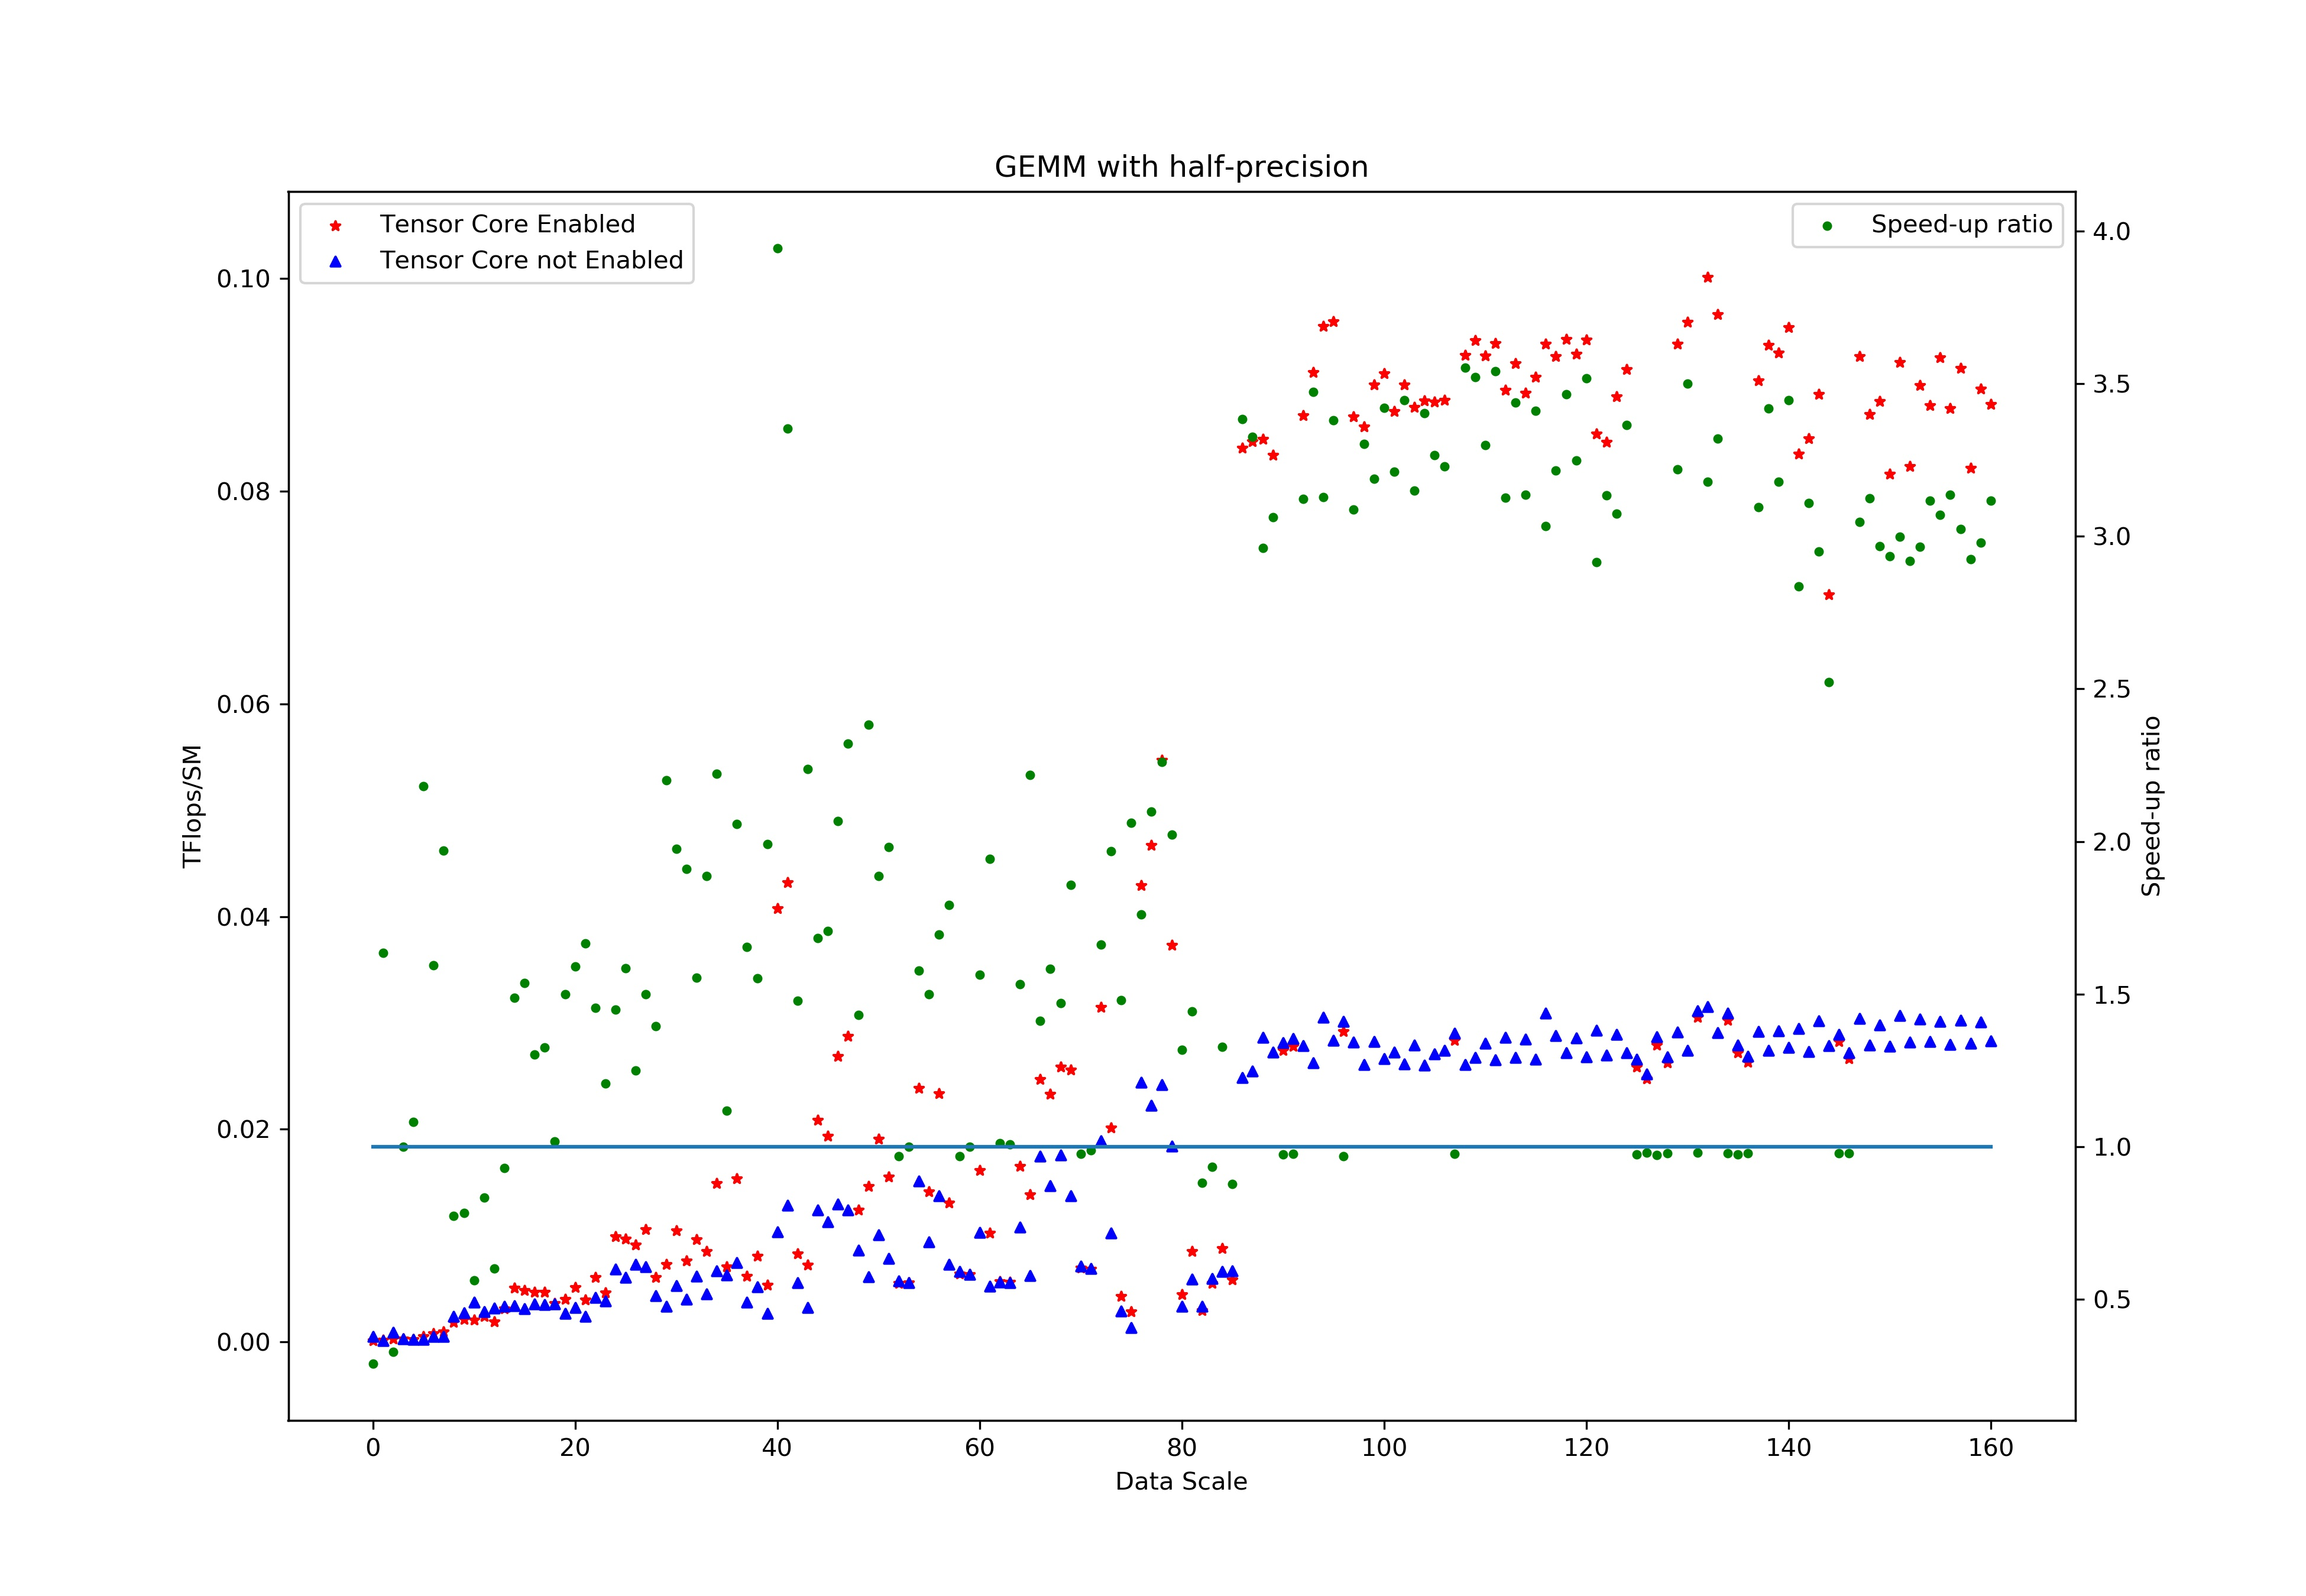
\includegraphics[width=7.5cm]{figures/GEMM-Half-TF.jpg}
	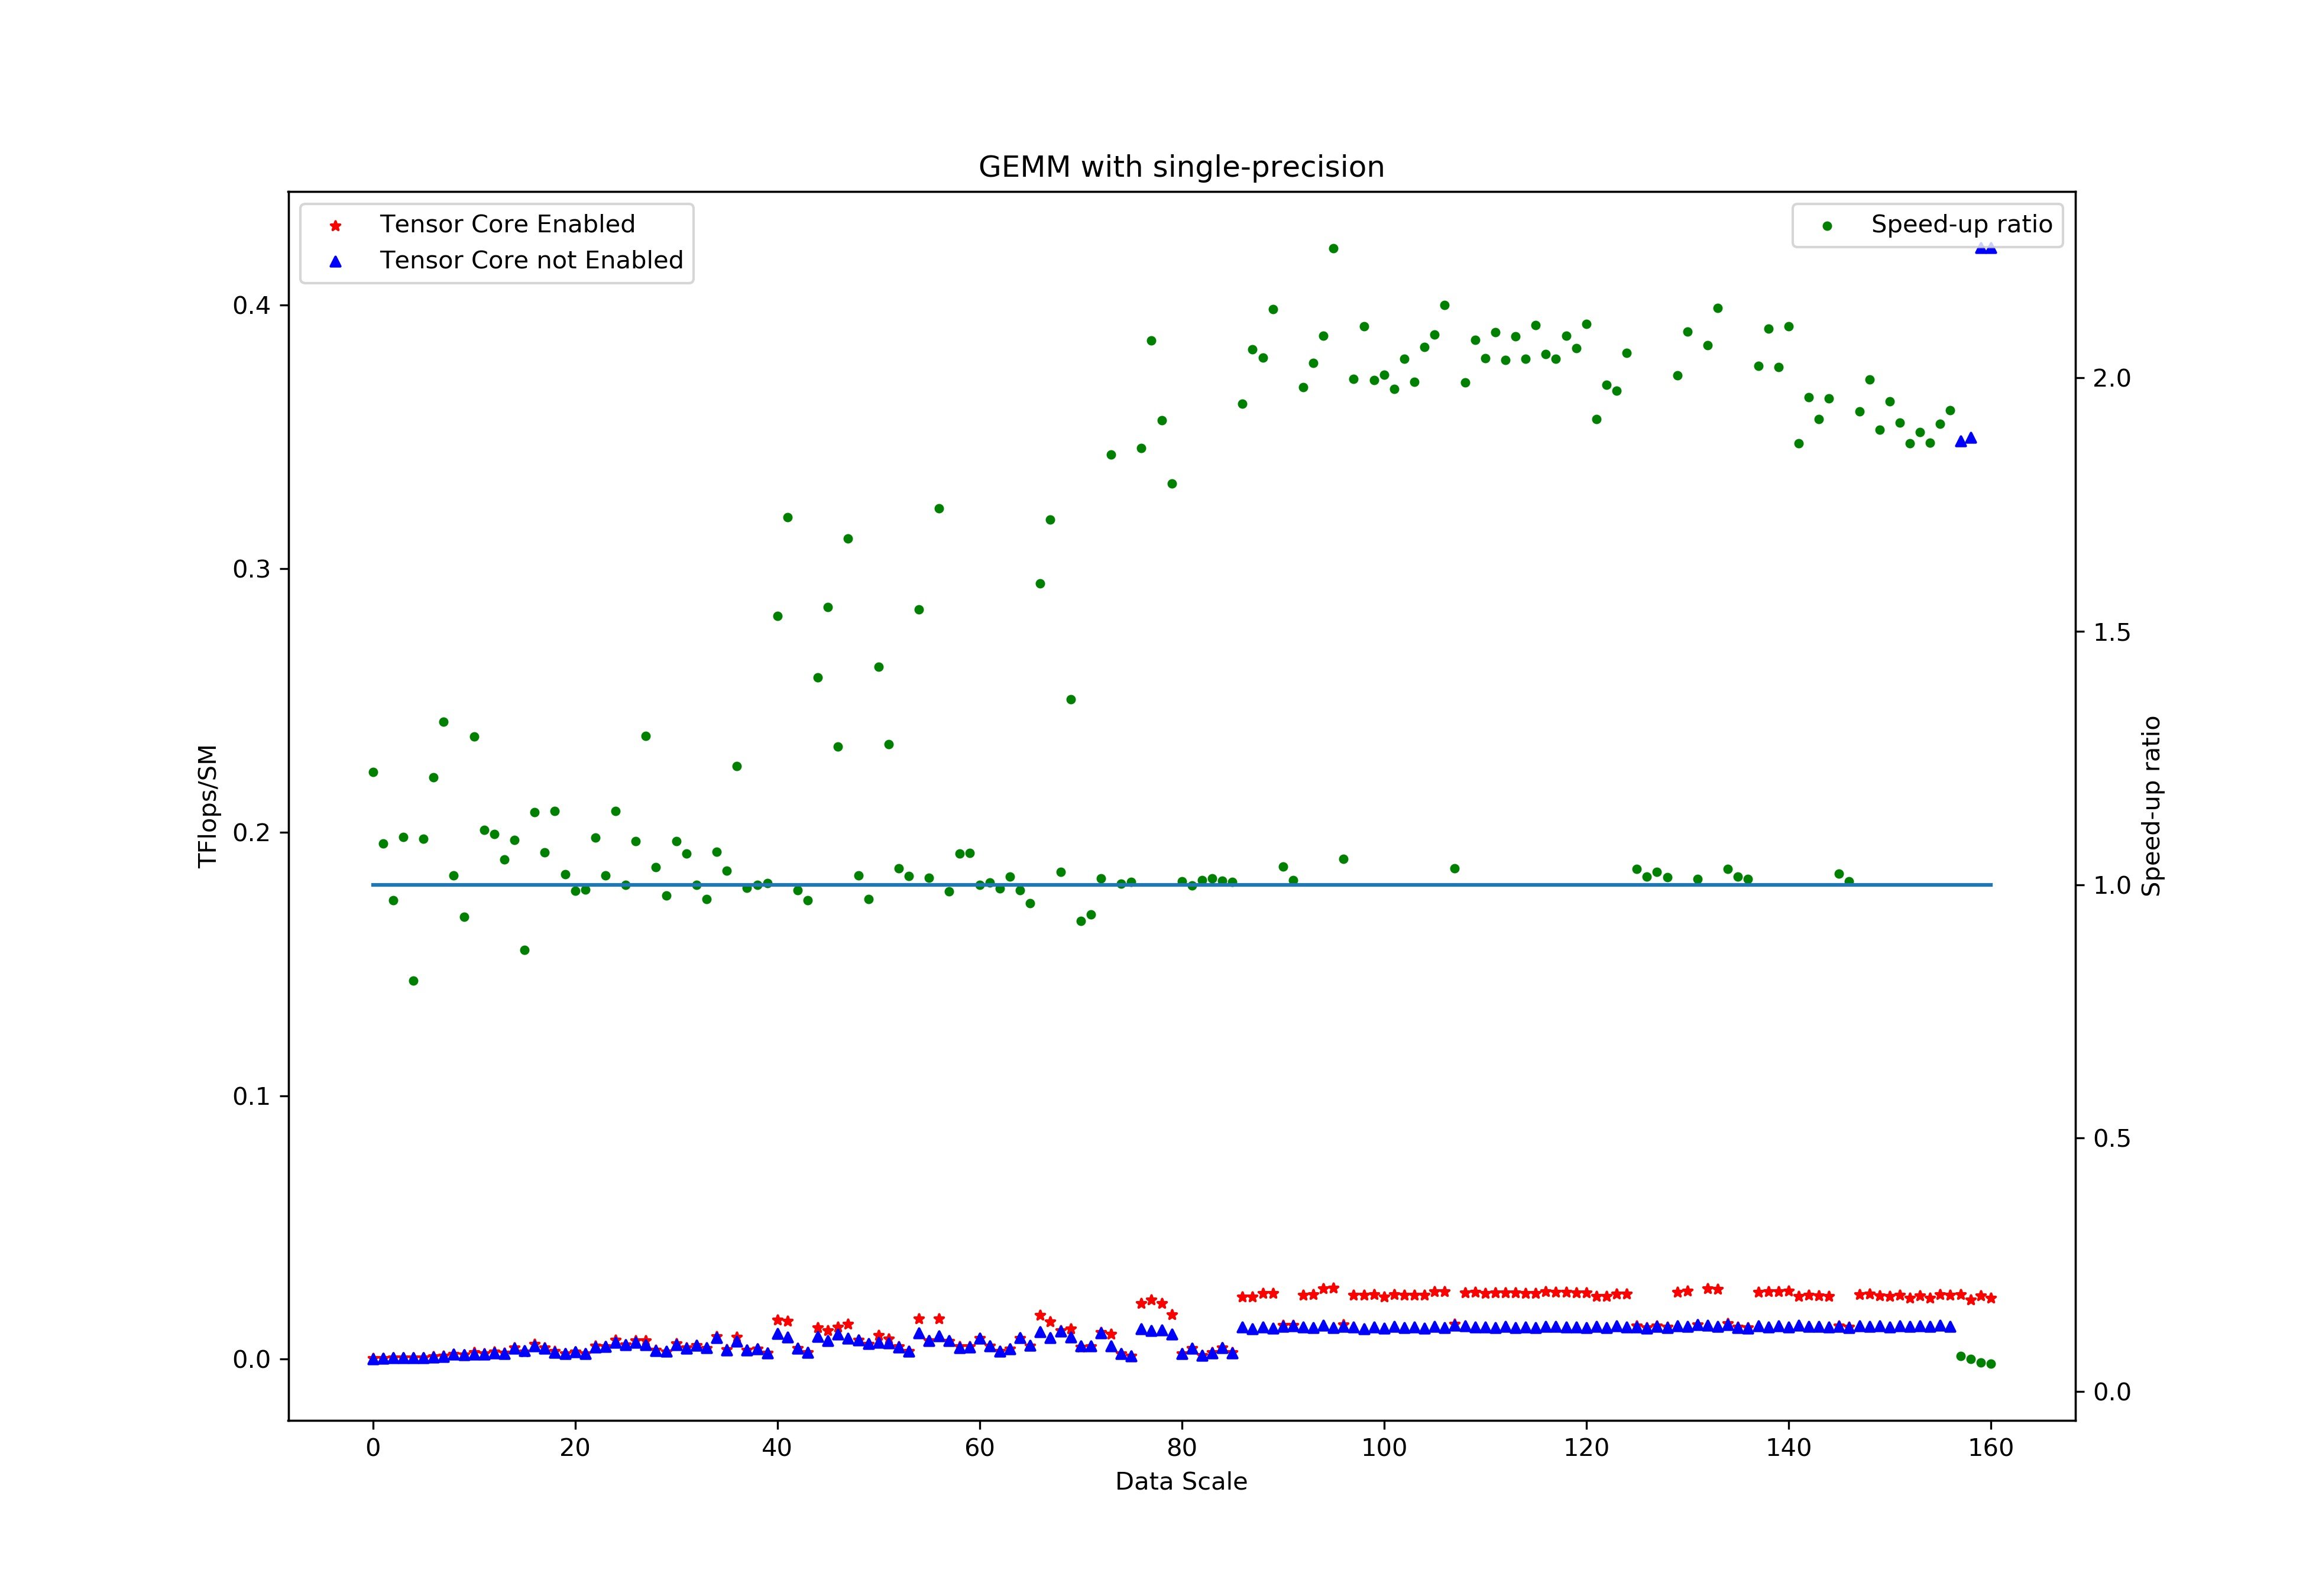
\includegraphics[width=7.5cm]{figures/GEMM-Single-TF.jpg}
	\renewcommand{\thefigure}{\arabic{section}-\arabic{figure} }
	\renewcommand{\figurename}{图}
	\caption{半精度/单精度GEMM性能}
	\addtocounter{figure}{-1}
	\renewcommand{\thefigure}{\arabic{section}-\arabic{figure} }
	\renewcommand{\figurename}{Figure}
	\caption{Performance of GEMM at Half and Single}
	\label{Fig-PerfGemm}
\end{figure}
\begin{figure}
	\centering
	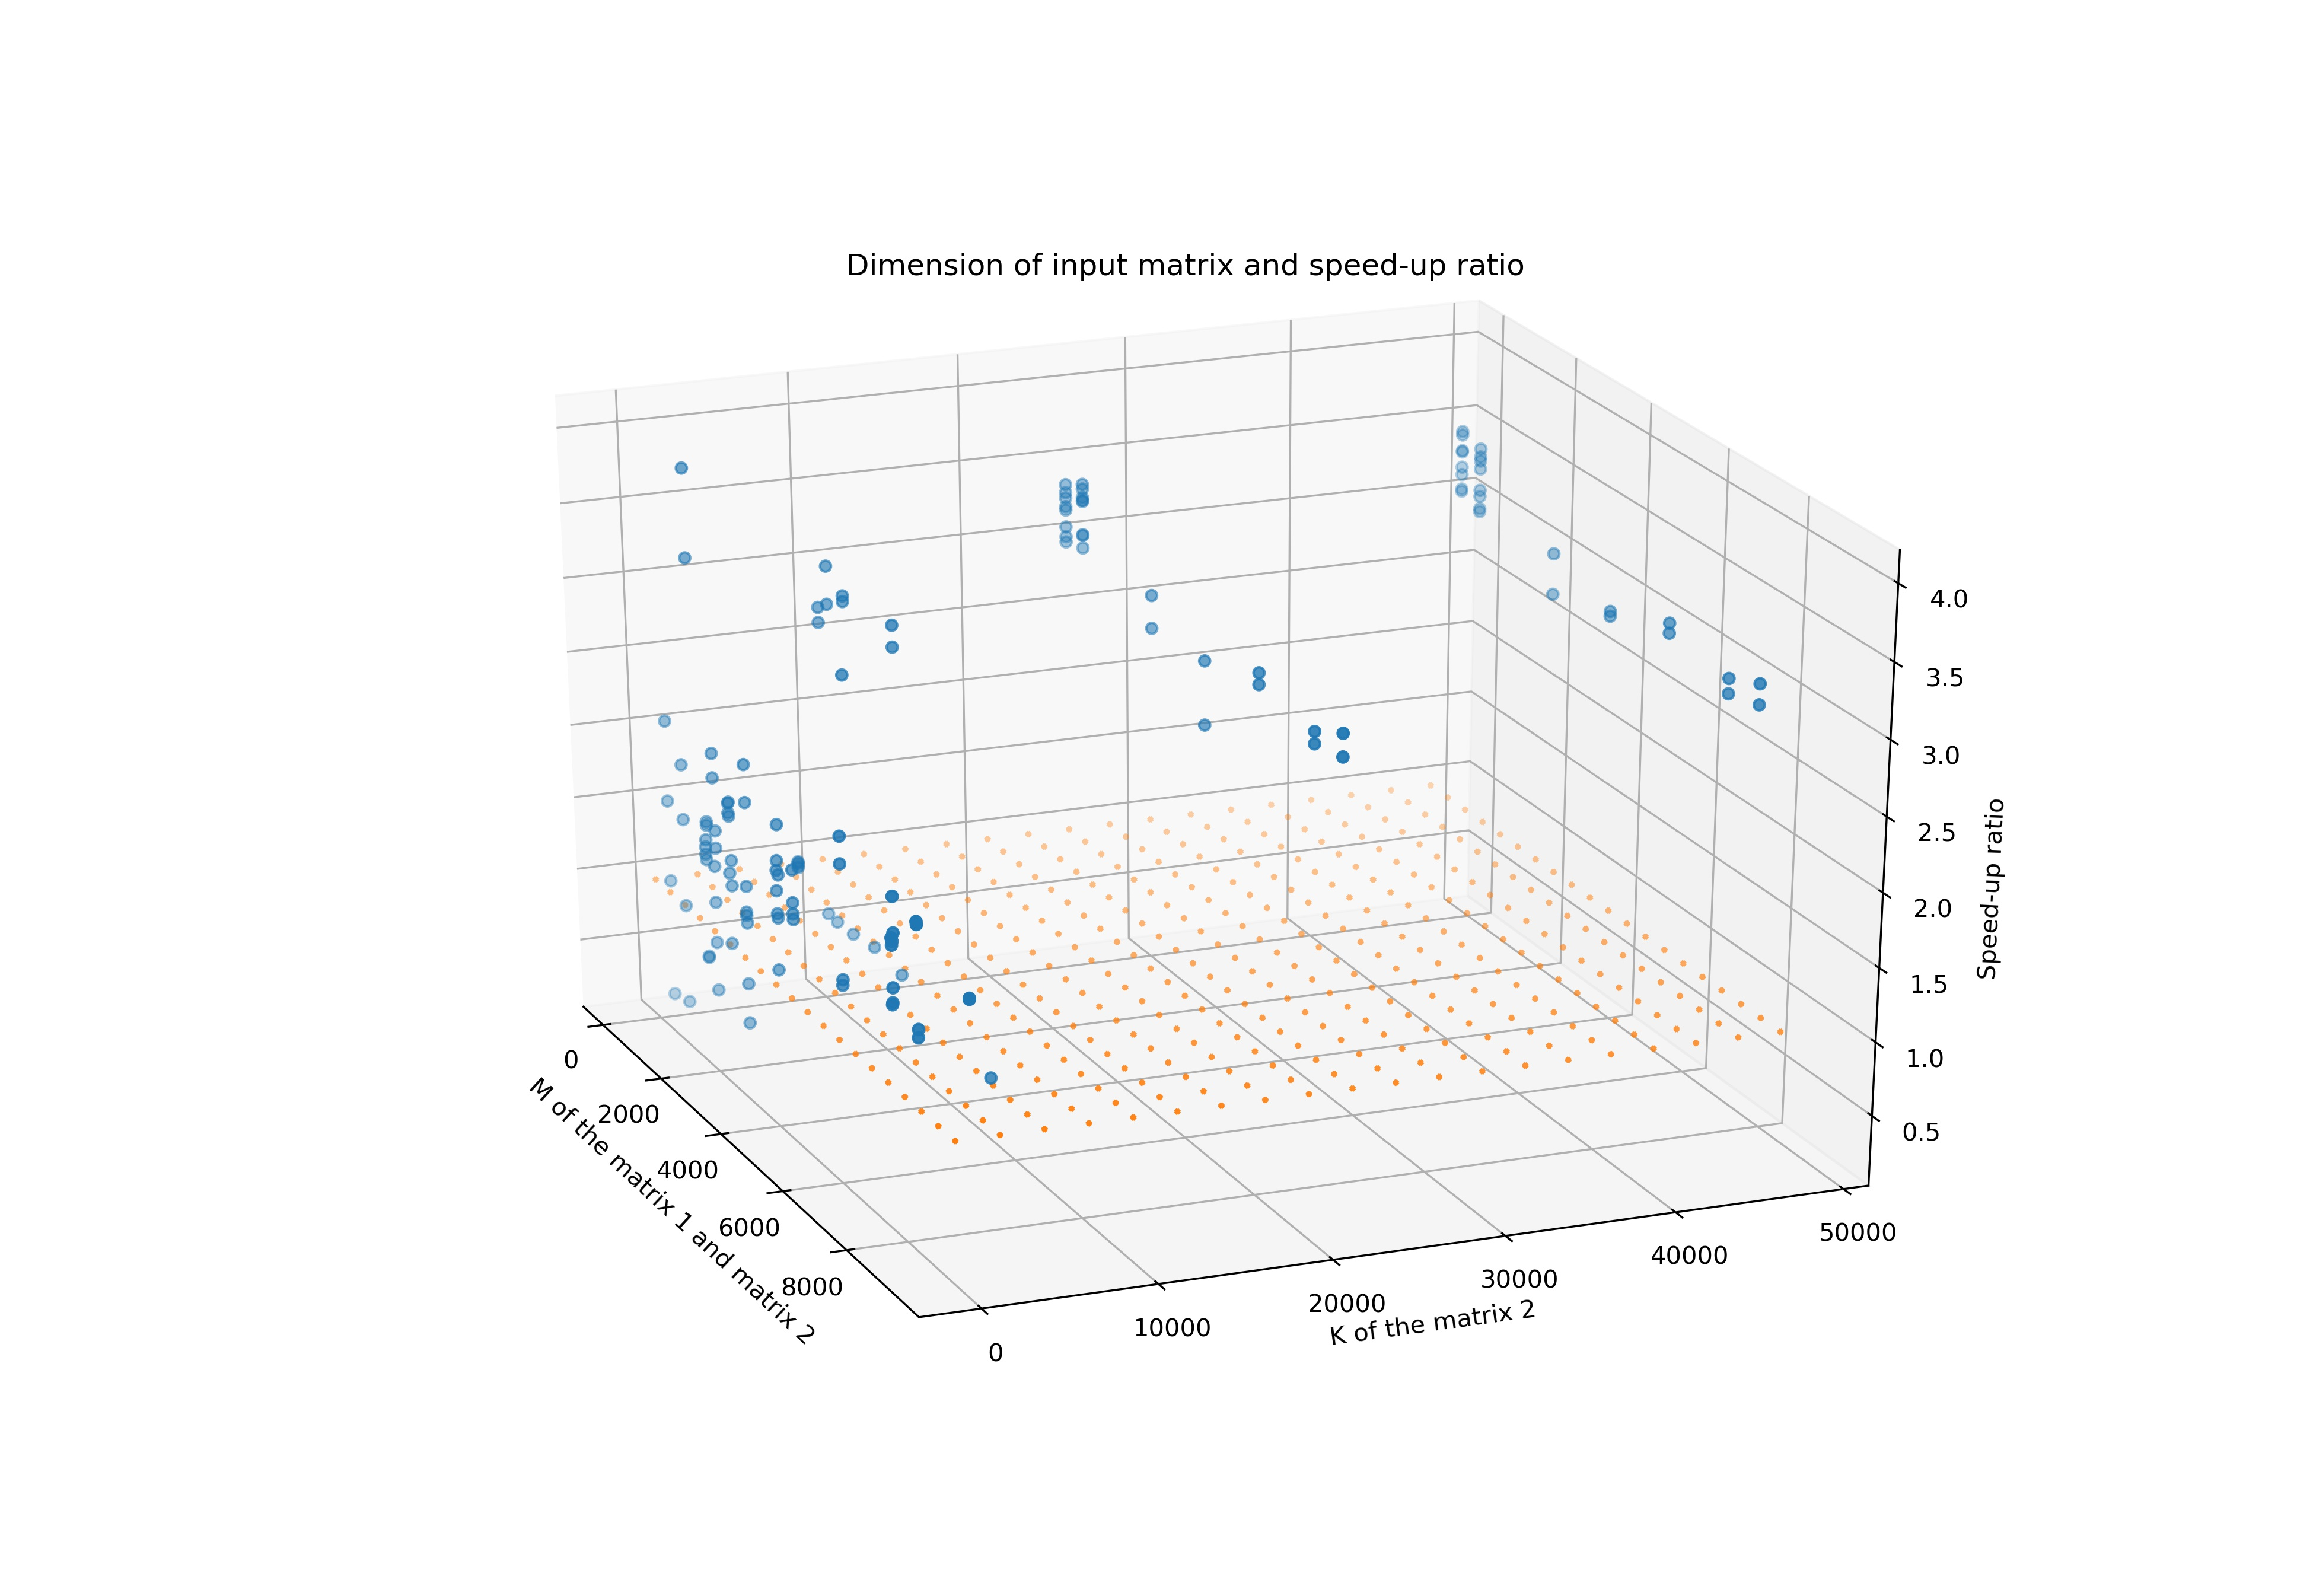
\includegraphics[width=7.5cm]{figures/GEMM_MK.jpg}
	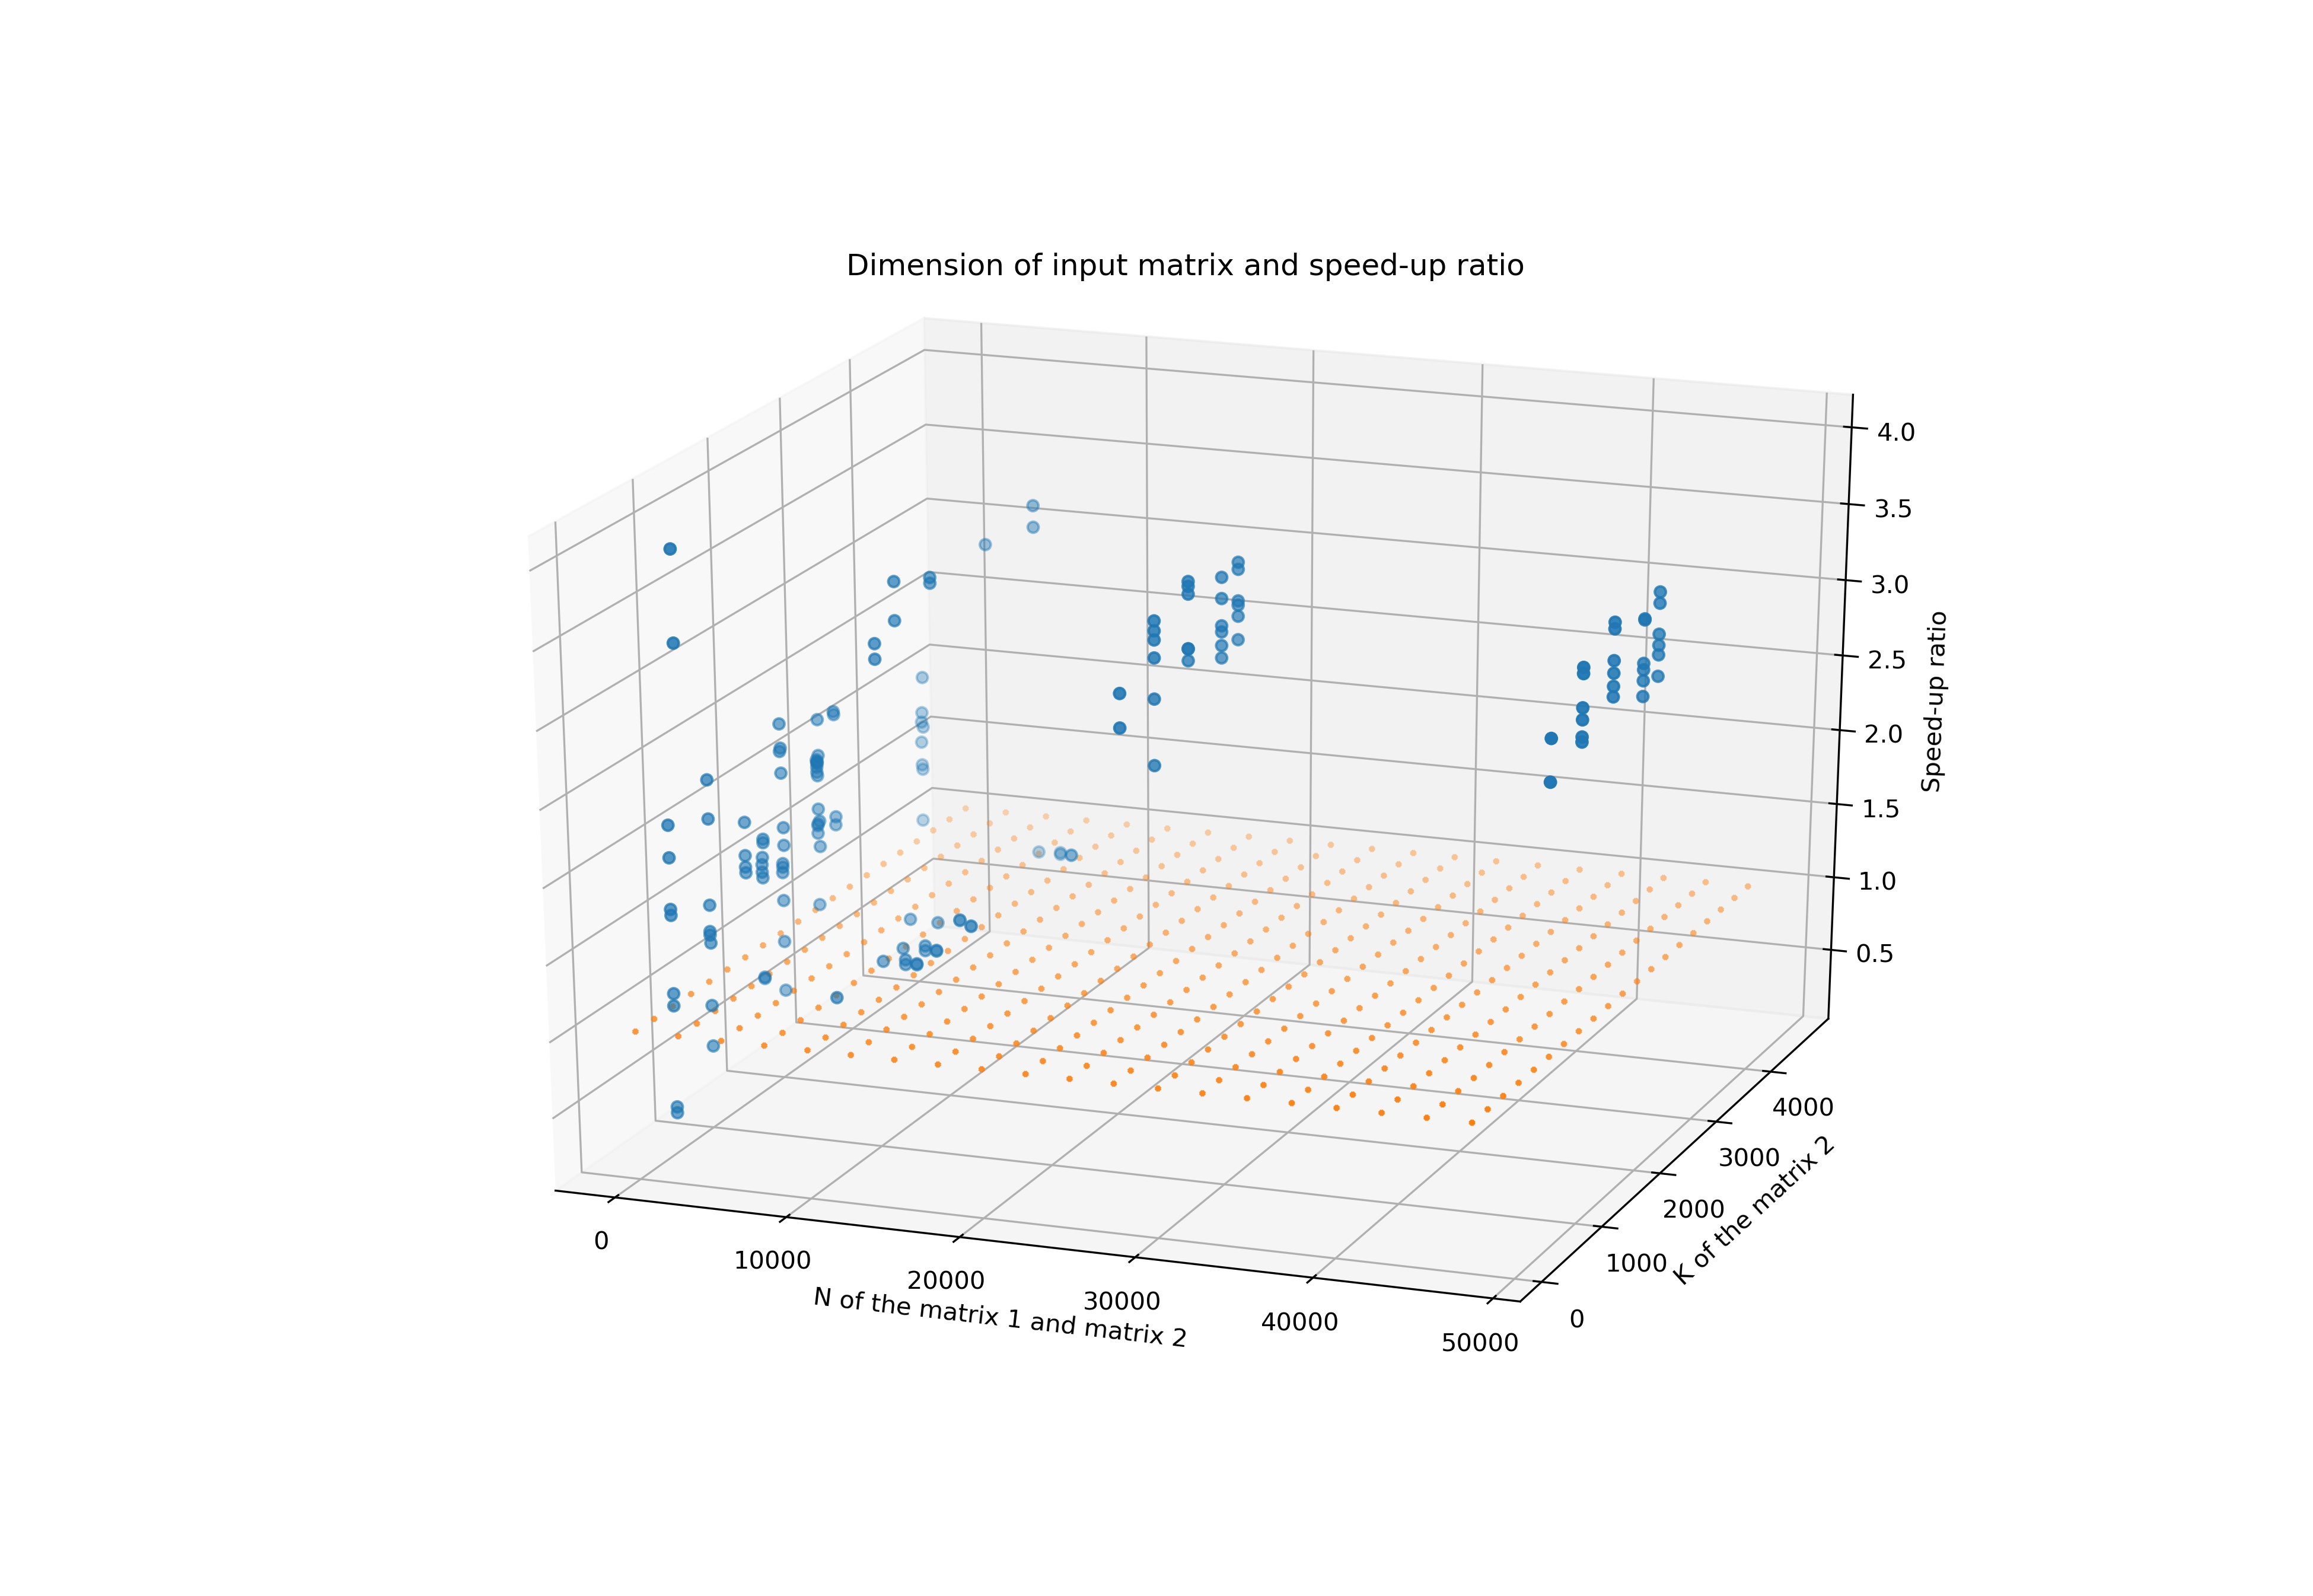
\includegraphics[width=7.5cm]{figures/GEMM_NK.jpg}\\
	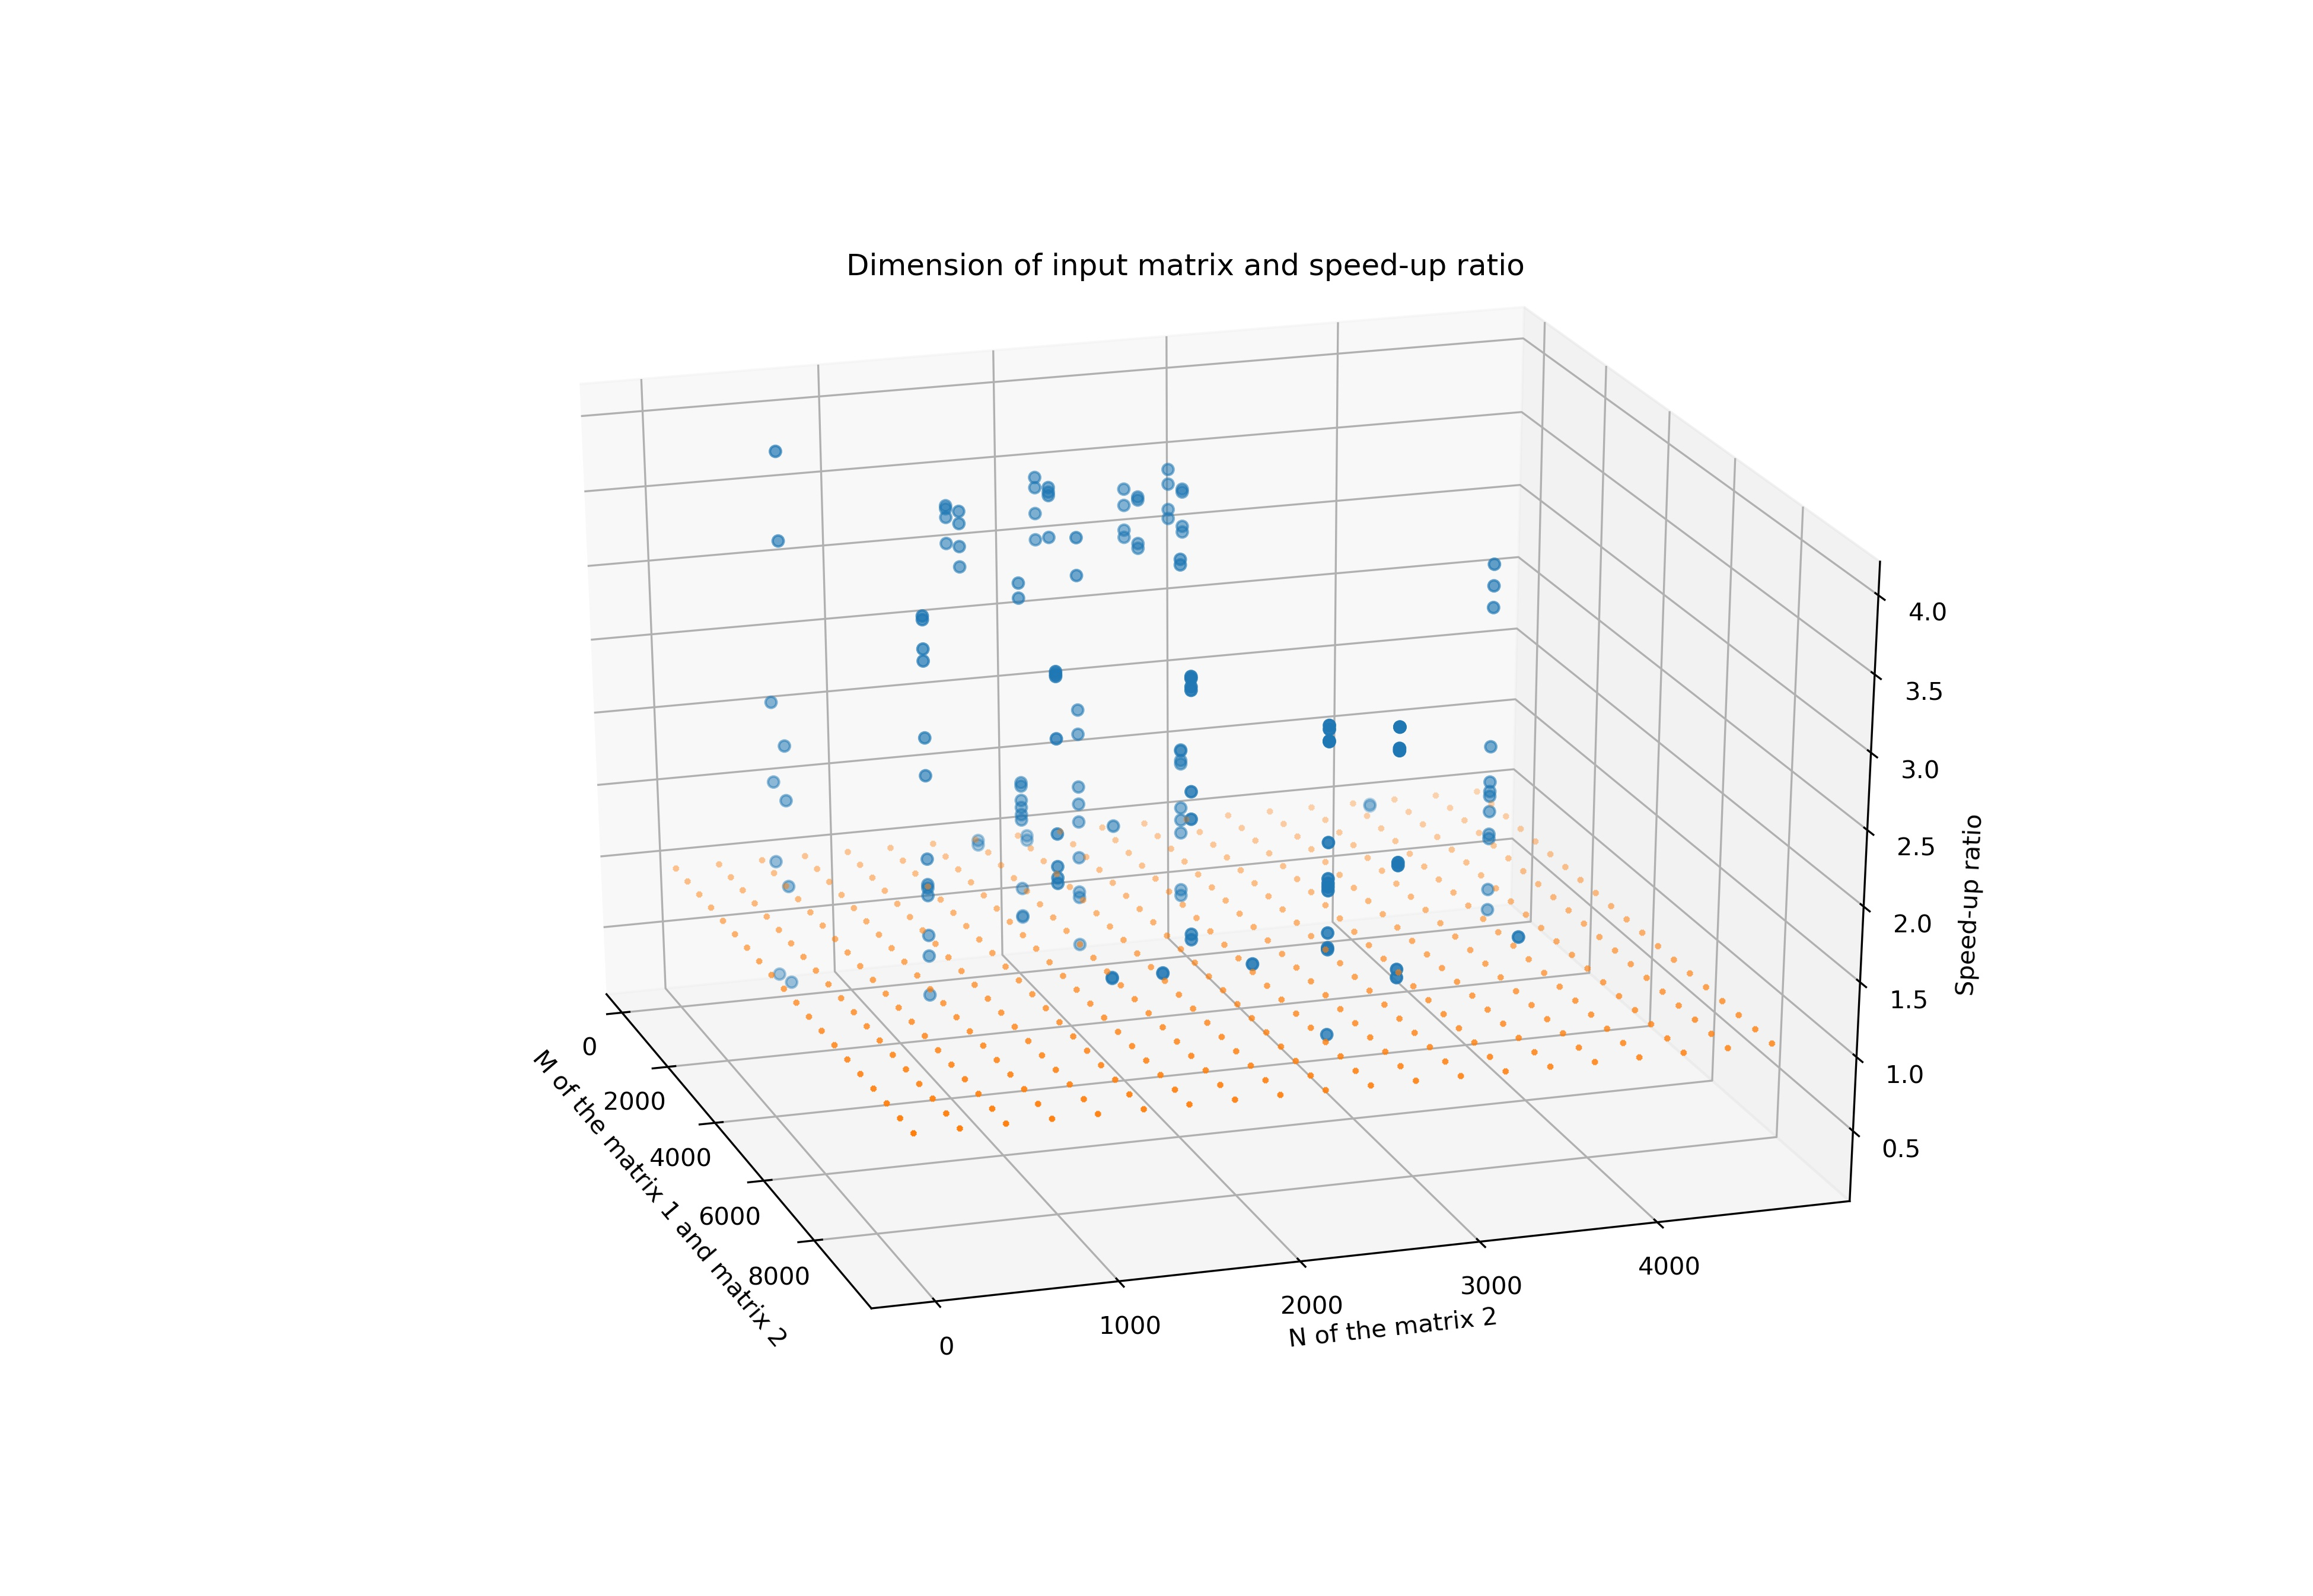
\includegraphics[width=7.5cm]{figures/GEMM_MN.jpg}
	\renewcommand{\thefigure}{\arabic{section}-\arabic{figure} }
	\renewcommand{\figurename}{图}
	\caption{输入矩阵维度与加速比的关系}
	\addtocounter{figure}{-1}
	\renewcommand{\thefigure}{\arabic{section}-\arabic{figure} }
	\renewcommand{\figurename}{Figure}
	\caption{Relationship of input matrix dimension and speed-up ratio}
	\label{Fig-MNKRatio}
\end{figure}
\begin{figure}
	\centering
	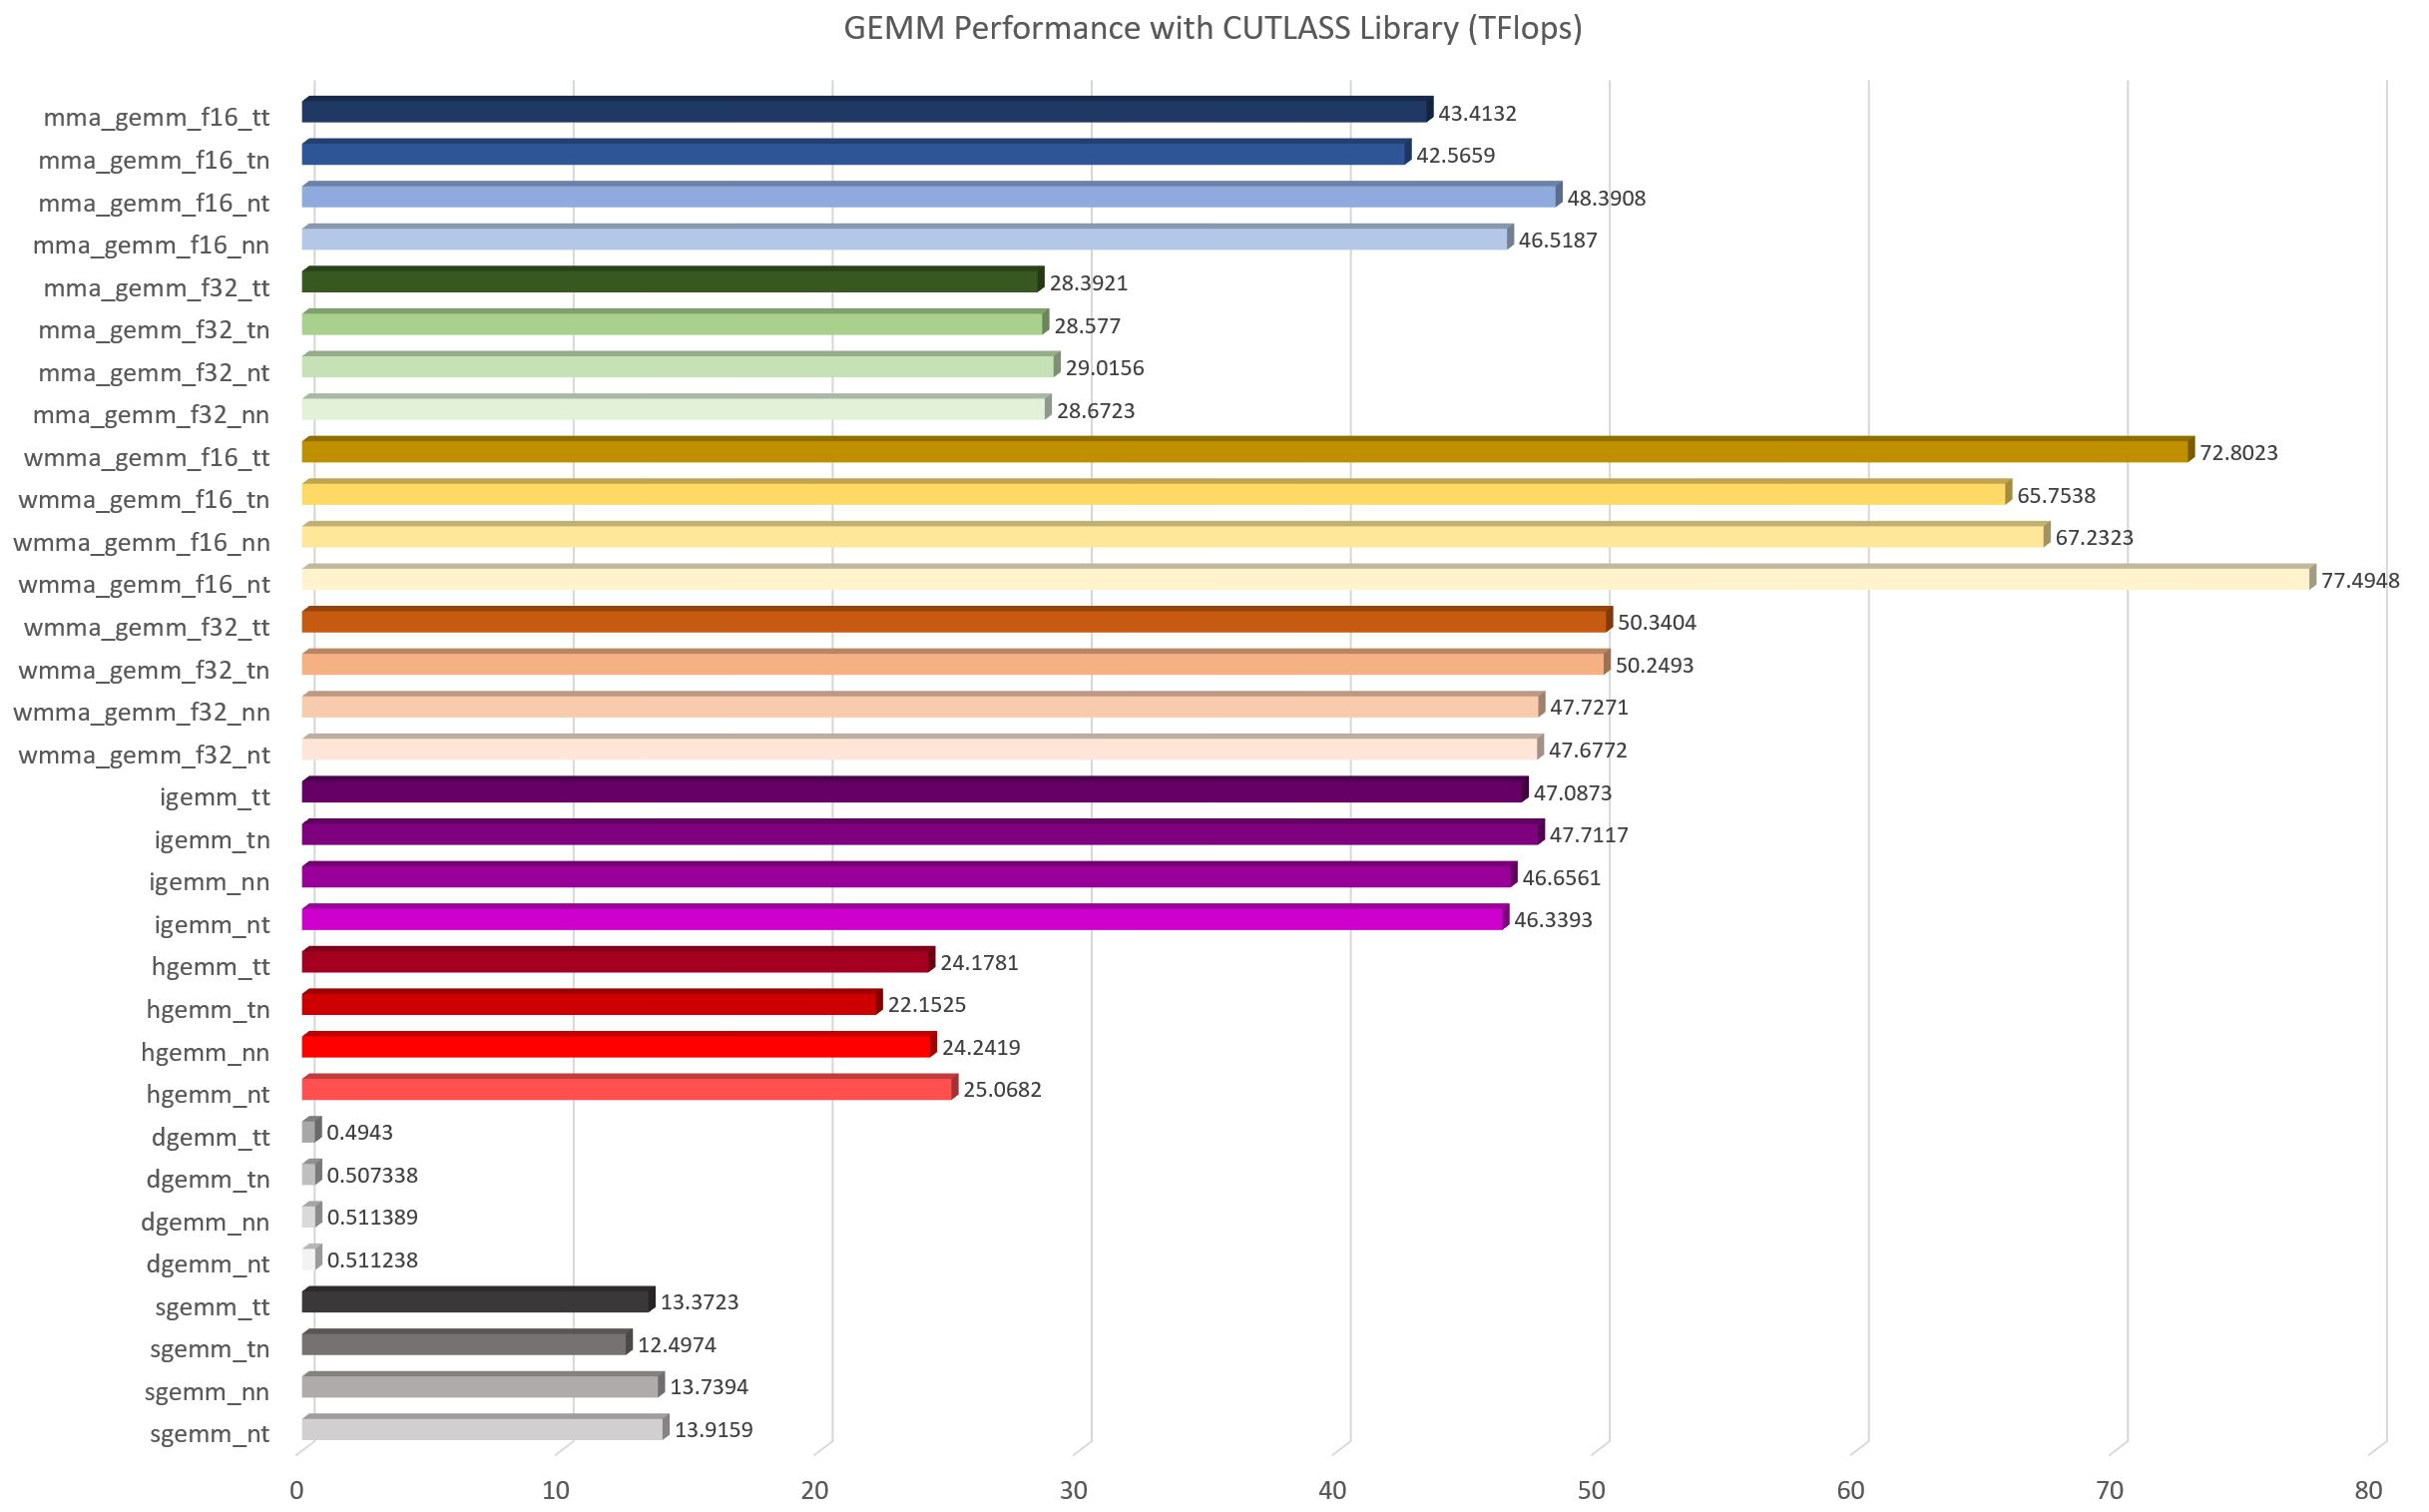
\includegraphics[width=15cm]{figures/CUTLASSGEMM.jpg}
	\renewcommand{\thefigure}{\arabic{section}-\arabic{figure} }
	\renewcommand{\figurename}{图}
	\caption{使用模板库测得的GEMM性能}
	\addtocounter{figure}{-1}
	\renewcommand{\thefigure}{\arabic{section}-\arabic{figure} }
	\renewcommand{\figurename}{Figure}
	\caption{GEMM Performance with CUTLASS}
	\label{Fig-GEMM-CUTLASS}
\end{figure}
\subparagraph{结果分析}
\paragraph{矩阵乘法运算}
\subparagraph{实验结果}
\subparagraph{结果分析}
\paragraph{卷积运算}
\subparagraph{实验结果}
\subparagraph{结果分析}
\paragraph{神经网络推理}
\subparagraph{实验结果}
\subparagraph{结果分析}
\subsubsection{基于CUDA源码的应用}
\paragraph{卷积神经网络}
\subparagraph{实验结果}
\subparagraph{结果分析}
\paragraph{并行支持向量机}
\subparagraph{实验结果}
\subparagraph{结果分析}
\subsubsection{基于TensorFlow框架的应用}
\subparagraph{实验结果}
\subparagraph{结果分析}